% !TEX TS-program = pdflatex
% !TEX encoding = UTF-8 Unicode

%************************************************
\chapter{Lo studio compositivo, tratti e indicazioni gestuali}
\label{chp:Lo studio compositivo, tratti e indicazioni gestuali}
%************************************************

\epigraph{Passa l'infinito di lì, passa la luce, non c'è bisogno di dipingere [...] invece tutti hanno pensato che io volessi distruggere: ma non è vero io ho costruito, non ho distrutto. \\ Lucio Fontana, \textit{Concetto Spaziale - Attese, 1961}}

Pensare di costruire un suono e al contempo distruggere tutto il passato solo grazie ad uno stralcio con la cultura precedente, penso sia un passo al quanto azzardato, nonché inutile. Il contatto con il passato non è soltanto un punto di passaggio nel quale fare tappa, ma diventa un cardine, un punto di slancio, con il quale argomentare qualunque percorso presente proiettato nel futuro che si va a ideare. \\
La notazione, se si parla di strumenti entrati ormai da centinaia di anni nella tradizione, dovrà essere pressoché classica e piena di quei piccoli accorgimenti che possano far interagire in maniera piena l'esecutore con lo strumento.

\section{Dal paragone all’indipendenza del suono}

Dopo aver effettuato le mie analisi di comparazione tra spettri armonici e inarmonici e aver individuato delle somiglianze e delle differenze all’interno dei due, ho anche notato nei miei studi di musicologia che alla base di molte ricerche musicali abbiamo soprattutto quest’idea di “comparazione” tra strumenti di liuteria classica e parti elettroniche o oggetti sonori a spettro inarmonico. Di base però l’idea di comparazione allontana, a mio parere, dal vero senso di interazione tra gli strumenti che dovrebbero essere semplicemente l’inizio di una ricerca personale sul suono. Non è più la ricerca di sembrare o apparire un suono quanto un altro, ma semplicemente lavorare su una proprio immagine spaziale e sonora. \\
L’interazione tra gli elementi dovrebbe essere un mezzo e non il fine del nostro lavoro compositivo. L’unione dei due è solo un ennesimo algoritmo che ci da la possibilità di creare e comporre la nostra musica. Quindi, non più una ricerca che vada ad investigare verso un \textit{merge} tra i segnali, o utilizzare una modulazione ad anello per avere una modulazione tale da poterla integrare nel metodo, ma avere un’idea ben chiara sul proprio processo compositivo che è l’unione di tutti questi mezzi verso un’idea compositiva attuabile e intellegibile, ben salda. \\
Mi riferisco alla possibilità di fare una musica dove sia intellegibile il pensiero compositivo, se questa possieda o no rugosità o un’armonia interna. \\
L’idea di utilizzare la microfonazione come una lente di ingrandimento sul suono, che viene catturato 

\section{La stesura della partitura}

In questi anni di conservatorio ho lavorato molto sulla stesura di partiture sempre più complesse ma che potessero allo stesso tempo essere di facile comprensione. Facili nel senso in cui ogni simbolo rappresentasse un gesto ben definito e se ci fossero più gesti sovrapposti, o un gesto che rendesse possibile più suoni, annotarli tramite specifici simboli. 
Ho quindi creato un corollario\footnote{vedi \textit{cap. 2}} come abbiamo prima osservato nel caso della molla, dove ogni rigo o parte di esso, rappresenta una parte del gesto e che siano semplici da intendere nella loro complessità di sovrapposizione. \\
Per quanto riguarda la notazione, cerco sempre di trovare dei trattati, come avviene per il primo dei miei due movimenti, dove ho inserito un numero finito di figure scritte nel \textit{II trattato Netti/Weiss}. Questa composizione vuole essere una ricerca tra tecniche estese dello strumento e connubio con un’elettronica alla base semplice sia a livello frequenziale che di algoritmica, proprio per unire una complessità esecutiva con una semplicità nell’elettronica che però rafforzi e ravvivi l’intenzione sullo strumento e la sua preponderante forza espressiva. Nella partitura, come si può notare nella figura a fine paragrafo, ci sono i multifonici per lo strumentista e al di sotto di questi, i vari campioni, collocati nel punto in cui sono collocati nel missato.
\begin{figure}

\begin{center}

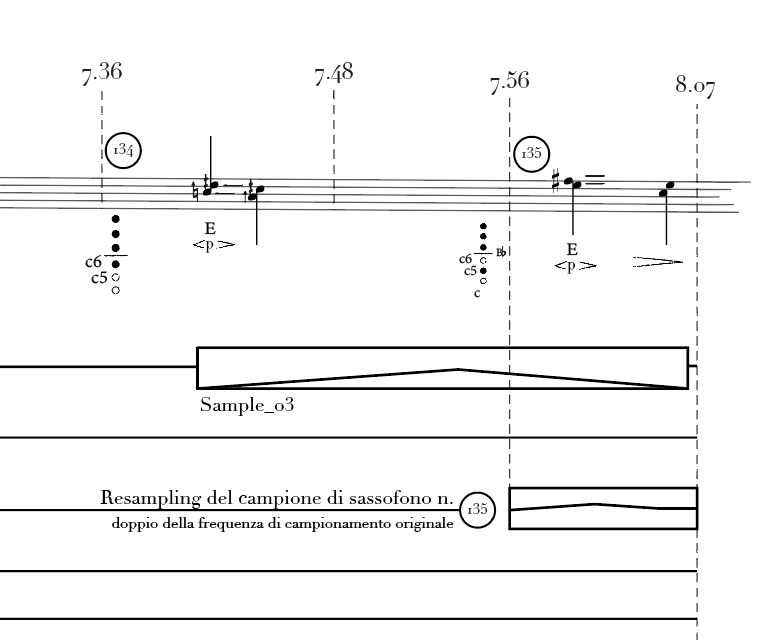
\includegraphics[width=1.\textwidth]{Partitura_particolare_01.jpeg}

\caption{Partitura: particolare}

\label{fig:01_Partitura_particolare_01}

\end{center}

\end{figure}


%************************************************

\subsection{L'utilizzo di una nuova notazione partituriale}

Come per lo \textbf{Sp.I.R.E.} (\textit{Spring installation Regulated and Electrify}), anche per Unamolla ho utilizzato uno nuova notazione e nuovi gesti, legati alla fisica dello strumento, ma senza allontanarmi troppo dall'eseguibilità del pezzo e l'eventuale riproduzione in futuro, da parte di chi, Unamolla, non la possiede, ma la può ricreare tramite lo schema e suonare, leggendo la partitura, da sé.

\begin{quotation}
Since music began to be notated, clearer distinctions between the work and its performance, and between the composer and performer, have emerged, representing multifarious views of the role of the performer.\footnote{Tanja Orning \textit{Pression} (a performance study) Norwegian Academy of MusicMusic Performance Research Copyright © 2012 Royal Northern College of Music Vol. 5}
\end{quotation}

La ricerca di nuove tipologie di notazione sta alla base della prassi strumentali, ovvero tecniche estese e tecniche compositive, ma anche nella creazione di una simbologia per l'elettronica, che risulti identificativa e allo stesso tempo espressiva. \\
Nella stesura del \textit{nastro magnetico} e nell'elaborazione ho preferito fare un catalogo dei miei campioni e dell'elaborazione di questi in modalità differenti, per il primo movimento e di elaborazione in tempo reale tramite filtri ed equalizzazioni in guadagno sullo strumento \textbf{Unamolla} per il secondo.

%************************************************

\section{Elaborazione del suono}

L'elaborazione del suono, dove aver preso in considerazione l'inquadramento storico e la capacità della ripresa microfonica come lente d'ingrandimento sul suono, diventa un vero e proprio prolungamento dell'esecuzione dello strumentista. Quindi, come accennato nell'introduzione, si ricerca un sentiero dove fondere l'elettronica e la parte eseguita su strumento. Ovviamente l'elaborazione ha necessità di esistere solo ed esclusivamente se viene utilizzata esclusivamente per scopi compositivi. I fini compositivi sono quindi la base del nostro lavoro e se ci troviamo a lavorare per una commissione, come avviene per \textit{L'albe nei varchi, come fuggir del susseguir d'incanti}, il primo dei tre varchi che compone il mio lavoro di tesi, ci dobbiamo scontrare con vari fattori. \\
In primo luogo sia l'elaborazione che l'eventuale "nastro magnetico\footnote{\textit{Nastro magnetico} va ad identificare una traccia audio sulla quale uno strumentista si trova a suonare. Identifico con nastro magnetico, semplicemente una traccia audio, solo per questioni storiche, non perché ci sia necessità reale di un nastro magnetico}" devono essere "trasportabili", ovvero devono essere reperibili eventualmente in una cartella presente in un \textit{cloud} nella rete, in comune con lo strumentista e con il registra, così da poter essere montata in fase preliminare e di esecuzione dal vivo senza la presenza fisica del compositore. \textit{L'albe nei varchi} rappresenta un brano su \textit{commissione}, il quale deve possedere, per essere eseguito con pochi intralci, queste caratteristiche:
\begin{itemize}
\item{\textit{Trasportabilità}: deve essere possibile trasporta la traccia audio su qualunque dispositivo e l'elaborazione avere diversi gradi: a seconda della tipologia di tecnico presente in regia, se non è presente il regista-compositore ci deve essere la possibilità di riprodurre la traccia su qualunque diffusione presente, anche, eventualmente, in mono.}
\item{\textit{Riproducibilità}: se si utilizzano software specifici, controllare che ogni parte del pacchetto che noi andiamo a creare sia di facile apertura in ogni personal computer, o addirittura, creare vari pacchetti per l'esecuzione, utilizzabili con programmi differenti. Uno schema algoritmico semplice e puntuale può essere la base per la ricostruzione in sede di sound-check e prove.}
\item{\textit{Eseguibilità}, ultima ma non inutile caratteristica, avere varie versioni, studiando prima i luoghi nei quali il brano verrà riprodotto, sarà decisivo.}
\end{itemize}